% This is the template for submission of abstracts to NetSci 2026 in Boston, USA.
% It is modified from NetSci2024, which was inspired by that of NetSci2016 and that of STATPHSY25.
% The editor of the booklet reserves the right to modify your submission.

% To process this file run LaTeX2e

% ******** DO NOT EDIT ****************
\documentclass[10pt]{article}
% \usepackage{mathptmx}
\usepackage[letterpaper,margin=20mm]{geometry}
\usepackage{graphicx}
\usepackage{lmodern}
\renewcommand{\familydefault}{\sfdefault}
\pagestyle{empty}
\setlength{\parskip}{0.25\baselineskip}
\renewcommand{\title}[1]{{\noindent\large\bfseries#1\medskip\\}}
\renewcommand{\author}[2]{{\noindent #1 \medskip\\ \noindent \small #2 \medskip\\}}
% *************************************

\begin{document}

% ********** USER DEFINED *************


% Enter title here
\title{Community Detection in Labeled Growing Hypergraphs}
\author{
% Enter author(s) here
Francis Cataldo,\textsuperscript{1}
Philip S. Chodrow\textsuperscript{1}
}
{
% Enter affiliation(s) here
1. Middlebury College, Middlebury, VT, USA
}

We consider a model of growing hypergraphs in which in which hyperedges form as noisy copies of prior hyperedges.
Our model extends prior work [1] by incorporating binary community node labels. 
The formation of new edges is affected by homophily with respect to these labels.
Unlike standard generative community detection methods which assume that edges form independently conditioned on node labels, our model instead explicitly assumes that new interactions are most likely to arrive between similar nodes \emph{which have previously iteracted}. 
This generative model is thus well-suited for community-detection for higher-order data sets collected from systems which may be reasonably believed to exhibit path-dependence, in which which interactions happen in the future are causally influenced by which interactions occurred in the past. 
This setting is common in many higher-order social and information systems; for example, in a network of scientific collaborations, whether a group of researchers collaborates on a new paper depends strongly on whether or not that same group, or some variant thereof, has collaborated in the past.
The community structures which result from this model are very different from those than which would be generated by standard stochastic blockmodel variants.

To perform community detection under this model, we develop a likelihood-based inference method.
Due to the computational complexity of computing the likelihood, we develop an approximation based on edge intersection sizes, which we show to have good empirical performance. 
We perform the maximization via simulated annealing. 
This approximated likelihood is highly correlated with the true labels of the graph, allowing the maximization of the approximate likelihood to yield an effective approximation of the true labels.
The latent-variable structure of this model also allows us to estimate the genealogy of edges, giving an approximate branching process describing the emergence of new interactions represented in the data. 

On synthetic data, we find that likelihood maximization in this model can result in much higher-fidelity reconstruction of ground-truth communities than standard methods such as Louvain modularity maximization (Fig. 1(a)-(b)). 
We also apply our methods to two classes of node-labeled data sets which do not obey standard community detection assumptions: legislate cosponsorship in the US congress (tagged by party affiliation) and co-authorship data from arXiv (tagged by inferred author gender).
In sum, our results indicate that methods for community detection in edge-dependent hypergraphs can outperform standard methods for some systems, and suggest future work for modeling and inference in such systems.

\begin{figure}[!h]
  \centering
  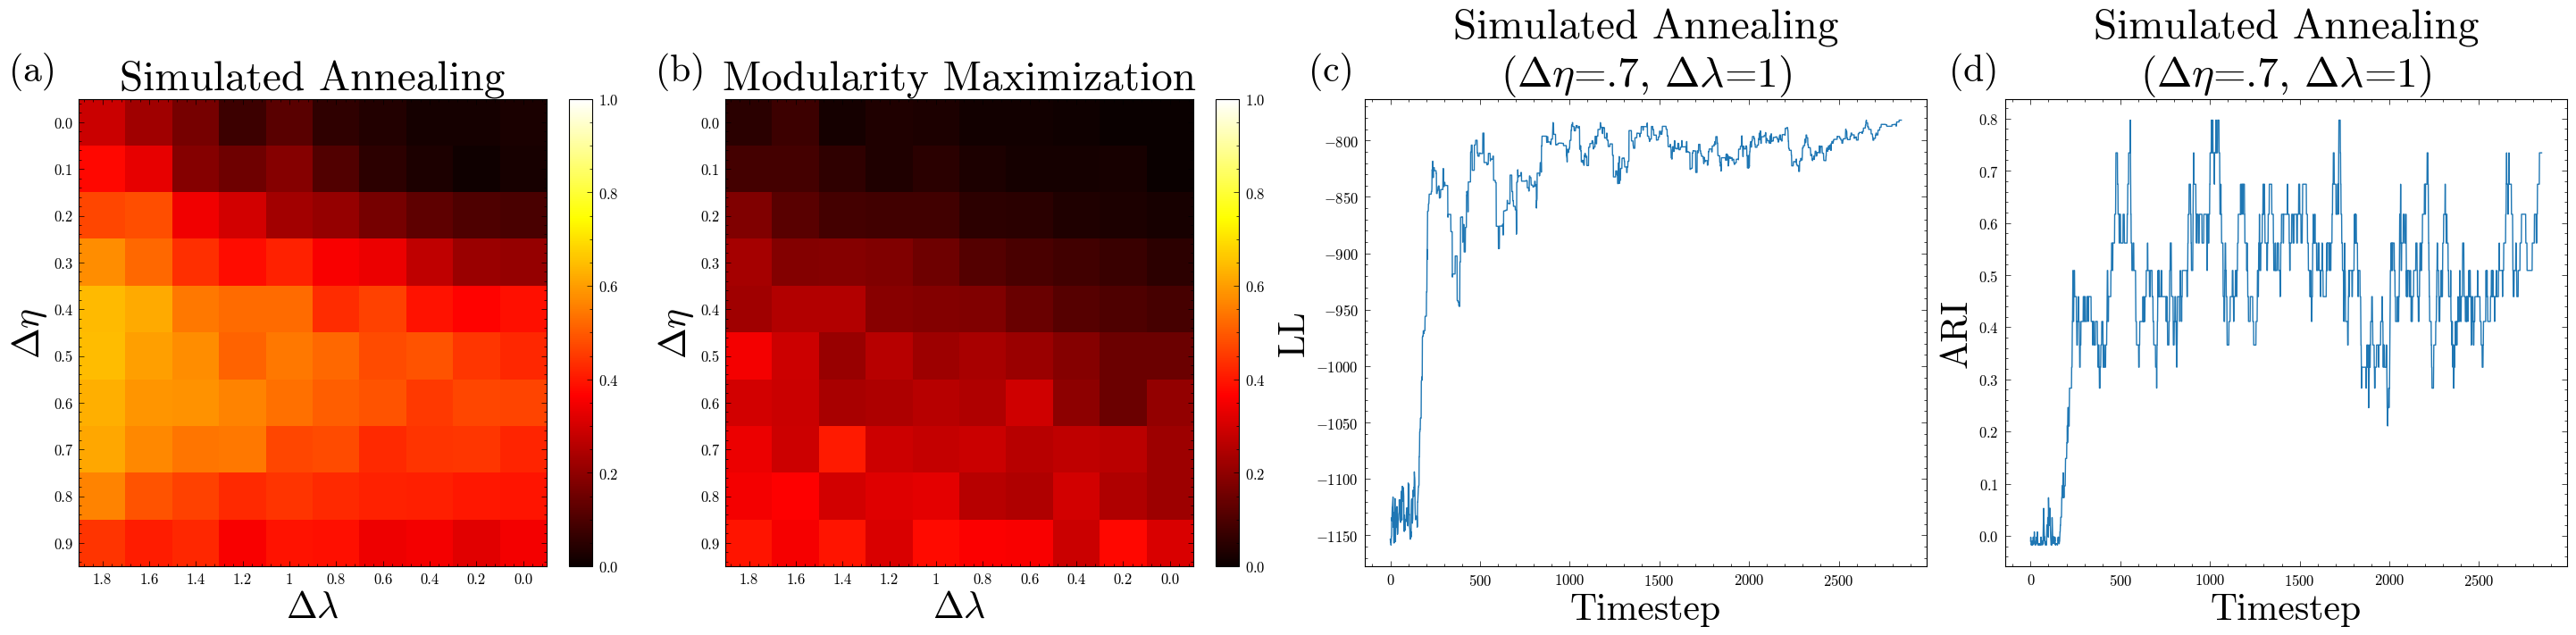
\includegraphics[width=\textwidth]{image.png}
  \caption{Performance of our maximum likelihood scheme on small synthetic data sets sampled from our model. (a): Adjusted Rand Index (ARI) between recovered labels and ground-truth labels as a function of the strength of homophily for different parameters; homophily is strongest on the lower left corner. Each pixel is an average over 10 initializations. 
  In each initialization, we begin with 26 starting nodes and edges. 
  We then grow the hypergraph for 50 timesteps, adding one edge per timestep, with number of nodes added depending on the choice of parameters. 
  (b): As in $a$, using Louvain modularity maximization instead. (c)-(d): Evolution of the log-likelihood and adjusted Rand Index against ground truth over algorithmic timesteps in one sample run.}
\end{figure}

\bigskip
{\small
\noindent[1] He, Chodrow, and Mucha. (2025) ``Edge Correlations and Link Prediction in Growing Hypergraphs.'' \emph{Physical Review E}.
}

% *************************************
\end{document}